\section{Woche 15 - CSAF-Workshop beim BSI} \label{sec:bericht-wo-15}

% 2023-12-11 bis 2023-12-15

\lweekdaymarginpar{\weekdayMondayShort\ - \weekdayWednesdayShort}

Die Woche begann ich mit der Recherche zu CSAF, wobei ich mit der offiziellen Dokumentation\footnote{\url{https://docs.oasis-open.org/csaf/csaf/v2.0/os/csaf-v2.0-os.html}} begann.
Den Großteil der Zeit habe ich mich mit den JSON-Strukturen, Rollen der Teilnehmer, dem Produkt-Matching und den anderen Konzepten, die hinter CSAF stehen, beschäftigt.
Mir fielen einige Unterschiede zu anderen Standards auf, wie zum Beispiel, dass CSAF nicht nur das Format der Security Advisories definiert, sondern auch deren Veröffentlichung, Bereitstellung, Aktualisierung und Verarbeitung durch Endnutzer.
Diese Erkenntnisse hielt ich in einem Wiki-Eintrag fest und bereitete mich Mittwoch auf die Reise vor.

\sweekdaymarginpar{\weekdayThursdayLong}

Donnerstagmorgen reiste ich früh um 5:45 mit dem ICE zum Information Security Hub (ISH) des BSI am Flughafen München, wo der Workshop stattfand (Abbildung \ref{fig:yan-ish-csaf-muenchen}).

\begin{figure}[htbp] % here, top, bottom, separate page
    \centering
    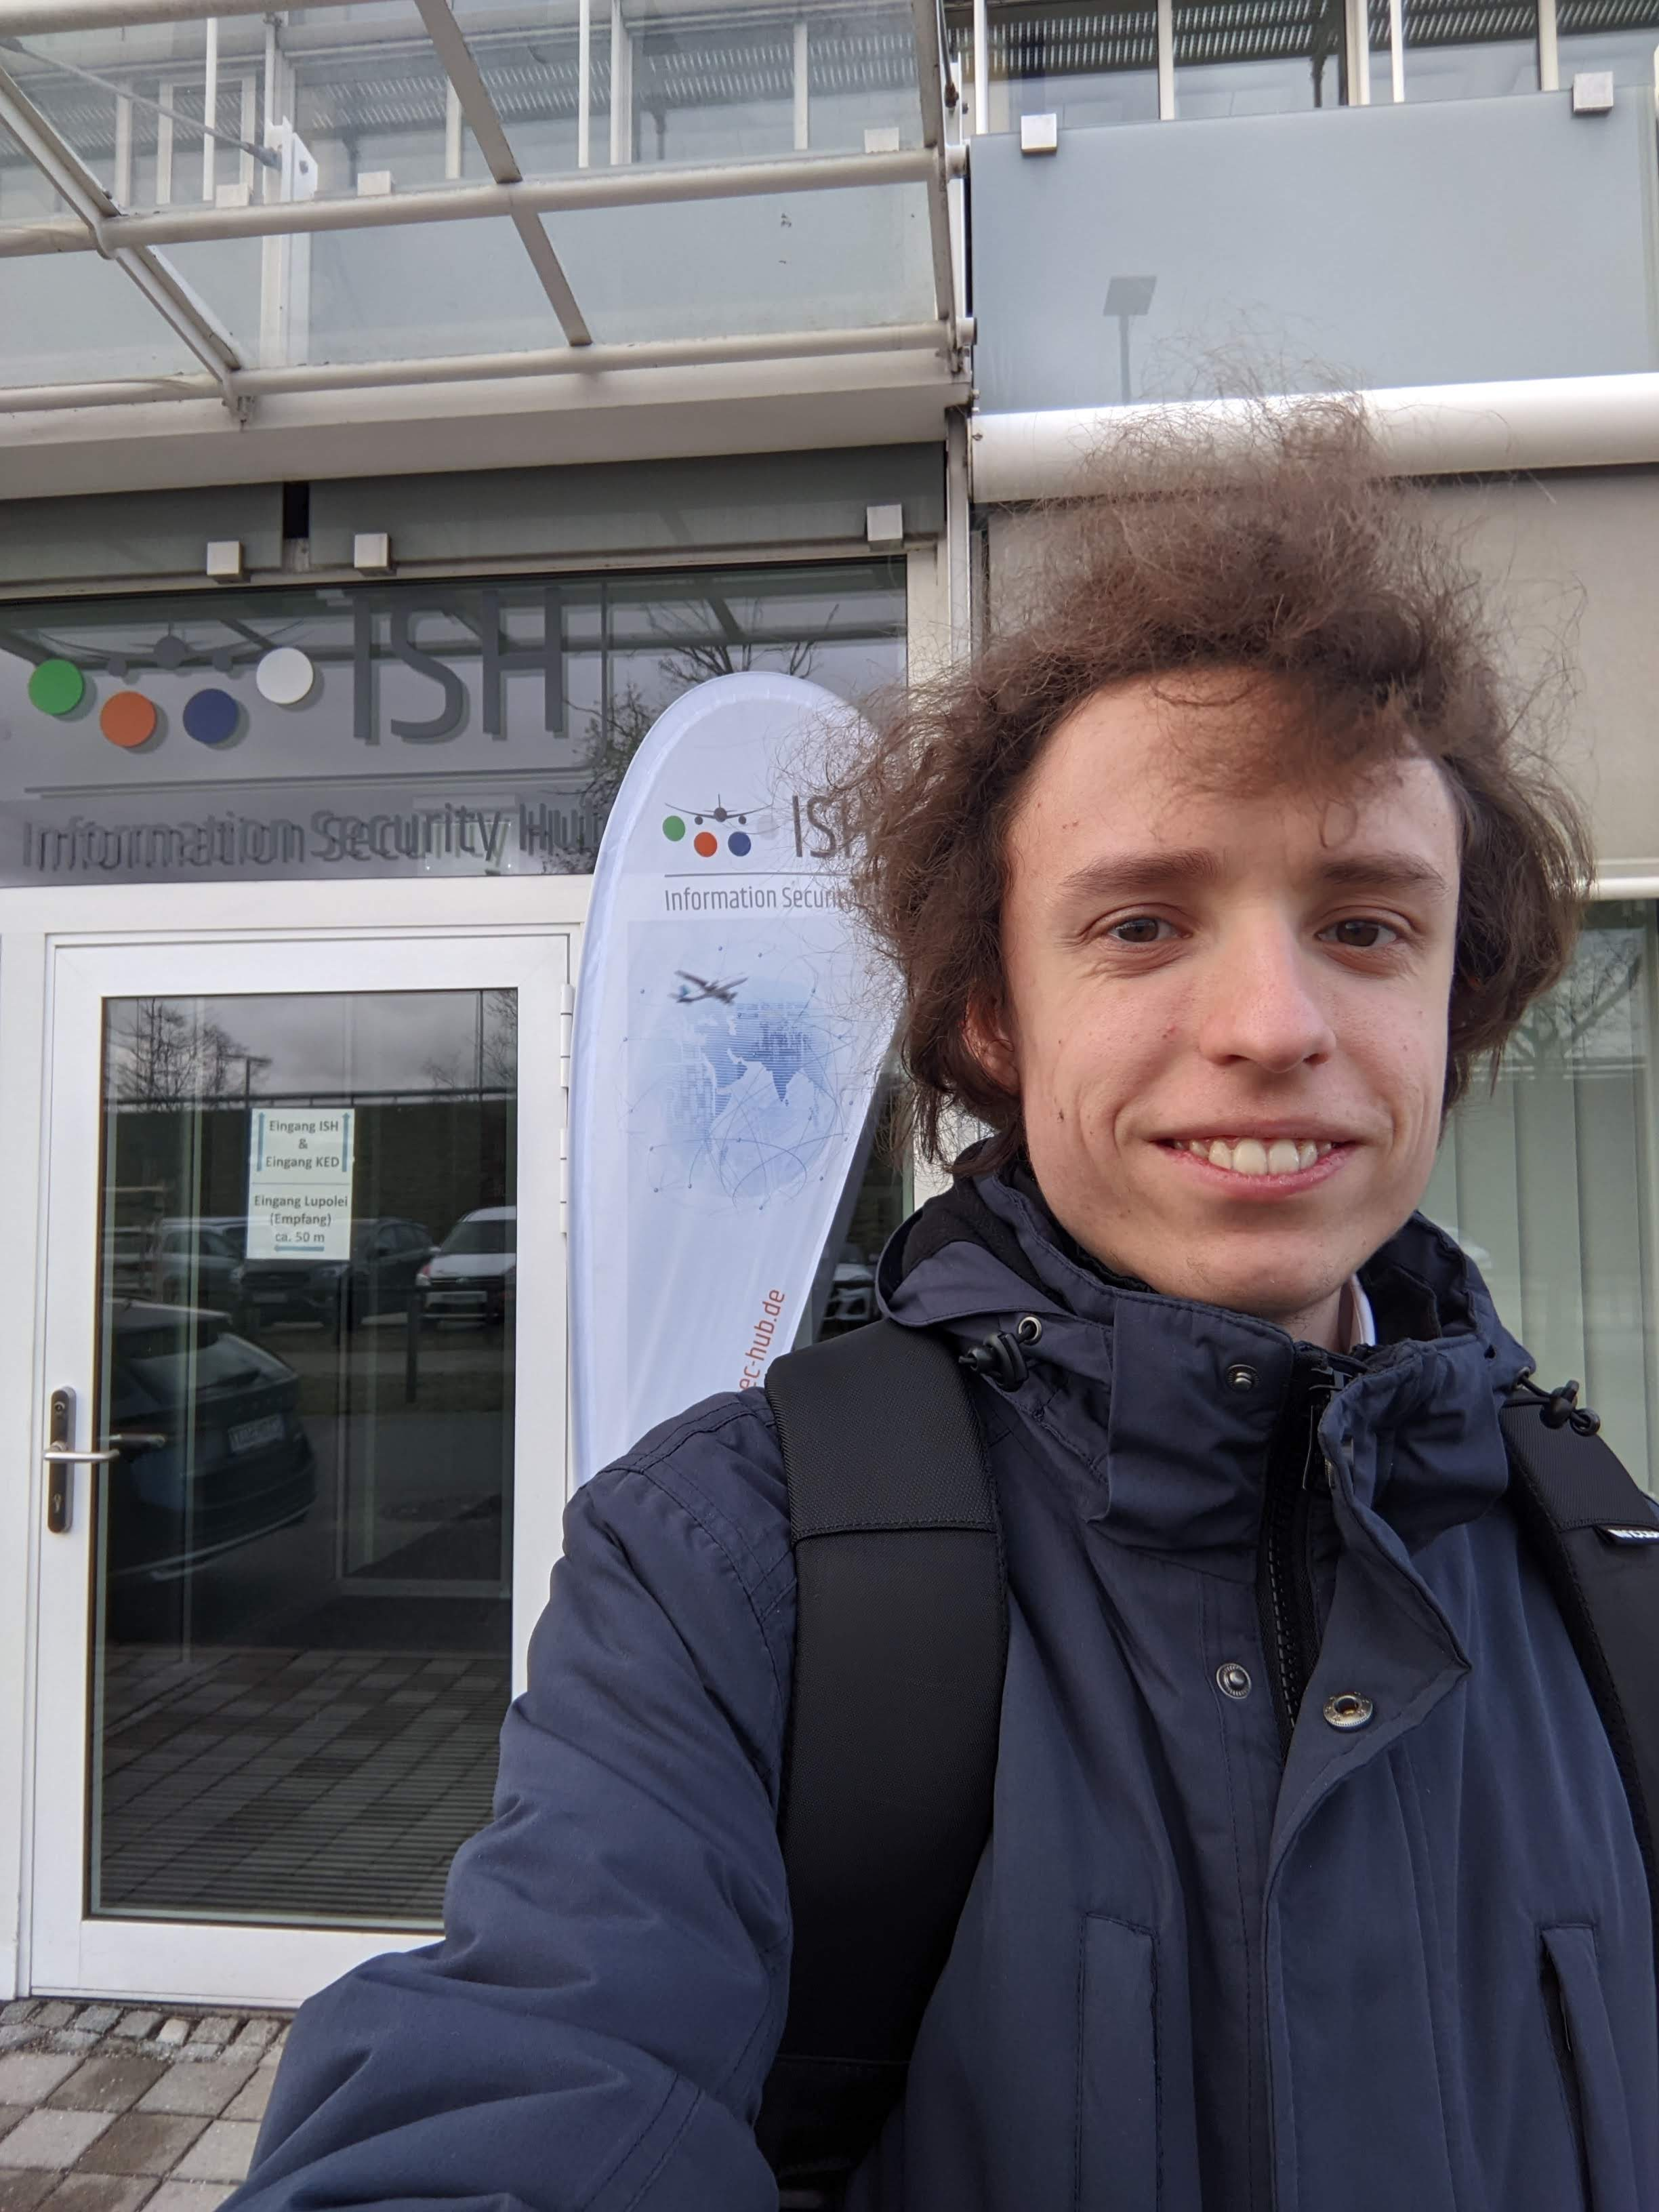
\includegraphics[width=0.4\textwidth, keepaspectratio]{res/img/2023-12-14-yan-vor-dem-ish-muenchen}
    \caption{Vor dem \qt{Information Security Hub} am Münchner Flughafen}
    \label{fig:yan-ish-csaf-muenchen}
\end{figure}

Vor dem Workshop nutzte ich die Gelegenheit, mich mit anderen Teilnehmern von Bosch und anderen Unternehmen auszutauschen.
Der Workshop selbst war eine Mischung aus theoretischen Präsentationen und praktischen Übungen.
Es ging um die Begriffe, Rollen und Abläufe, aber auch um das tatsächliche Einsetzen der bereitgestellten Tools, dem eigenen erstellen von Security Advisories und dem Veröffentlichen dieser.
Besonders interessant waren für mich die Diskussionen über die Produktidentifikation und dem CVSS-Standard.
Nach dem Workshop und weiteren Gesprächen am abschließenden Buffet beendete ich den Tag mit einem Telefonat mit meinem Chef.

\sweekdaymarginpar{\weekdayFridayLong}

Freitag setzte ich die Teilnahme am Workshop fort, heute war der Fokus auf der praktischen Anwendung des CSAF-Standards.
Ich konnte, nachdem ich die Aufgaben recht schnell abschließen konnte, anderen Teilnehmern dabei helfen, die weniger Informatiker sind als Planer und Manager.
Nach dem Workshop und abschließenden Gesprächen machte ich mich auf den Heimweg und kam sogar dank einer früheren Verbindung schneller nach Hause.
Meine ausführlichen Notizen und Überlegungen würde ich in der folgenden Woche präsentieren.
